\chapter{Specifica dei casi d'uso}

\section{Introduzione}
In questo documento sono analizzati ed elencati gli attori ed i casi d'uso del sistema.
Scopo del documento è la dettagliata descrizione delle modalità di interazione tra le diverse entità presenti ed il sistema.
Ciò permetterà di mettere in evidenza eventuali conflitti tra i requisiti del sistema stesso.
Tale analisi e descrizione dei casi d'uso verrà presentata tramite grafici che seguono lo standard UML.

\noindent
Si utilizzeranno le seguenti convenzioni:
\begin{itemize}
	\item Nei casi in cui più attori possono accedere ad un determinato caso d’uso, ma quest'ultimo è rivolto principalmente ad un solo attore, non verranno elencati tutti gli altri.

	\item Non verranno riportati tutti gli attori che hanno accesso ad un determinato caso d'uso, ma solo l'attore più generico.
	
	\item Nei diagrammi dei casi d'uso non viene riportato l'identificatore del singolo caso d'uso ma solo il titolo, per facilitarne la lettura.
\end{itemize}

\section{Elenco degli attori}
Gli attori che interagiscono con il portale sono elencati di seguito:
\begin{itemize}
	\item \newListItem{att:visitatore}{\formattaAtt}{Visitatore}
	\item \newListItem{att:utente}{\formattaAtt}{Utente}
	\item \newListItem{att:produttore}{\formattaAtt}{Produttore}
	\item \newListItem{att:redattore}{\formattaAtt}{Redattore}
	\item \newListItem{att:assistente}{\formattaAtt}{Assistente}
	\item \newListItem{att:moderatore}{\formattaAtt}{Moderatore}
	\item \newListItem{att:amministratore}{\formattaAtt}{Amministratore}
	\item \newListItem{att:cms}{\formattaAtt}{CMS}
\end{itemize}
La gerarchia degli attori è mostrata nel seguente diagramma UML:
\begin{center}
   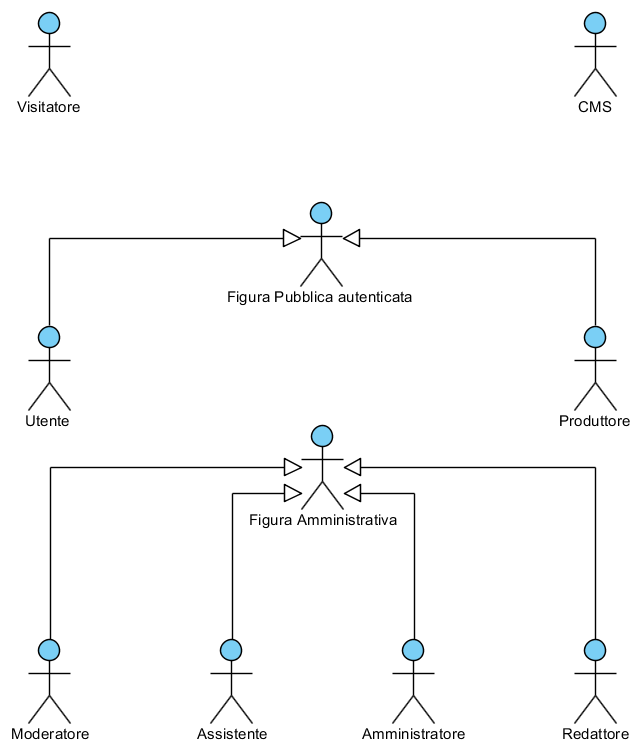
\includegraphics[width=\textwidth]{assets/visualParadigm/SchemaAttori}
\end{center}

\section{Specifica degli attori}
Gli attori che interagiscono con il portale sono descritti di seguito:
\attTab{att:visitatore}{-}{\glsdesc*{visitatore}}

\tabattvspace

\attTab{att:utente}{-}{\glsdesc*{utente}}

\tabattvspace

\attTab{att:produttore}{-}{\glsdesc*{produttore}}

\tabattvspace

\attTab{att:redattore}{\getTitletodesc{att:utente}}{\glsdesc*{redattore}}

\tabattvspace

\attTab{att:assistente}{\getTitletodesc{att:utente}}{\glsdesc*{assistente}}

\tabattvspace

\attTab{att:moderatore}{\getTitletodesc{att:utente}}{\glsdesc*{moderatore}}

\tabattvspace

\attTab{att:amministratore}{\getTitletodesc{att:utente}}{\glsdesc*{amministratore}}

\tabattvspace

\attTab{att:cms}{-}{\glsdesc*{cmsdef}}

\section{Identificativo dei casi d'uso} %(vengono usati per definire l'ID, non ha senso metterli dopo la struttura ID)
Di seguito è spiegato come interpretare l'identificativo dei casi d'uso:
\begin{center}
	\use{categoria}{caso}%{[sottoreq]}{[\dots]}
\end{center}

\noindent
Segue una descrizione di ogni campo utilizzato nell'identificatore:
\begin{itemize}
	\item La \campiIdReq{categoria} è una lettera utilizzata per raggruppare i casi d'uso con scopi simili.
	Le categorie sono le seguenti:
	\begin{enumerateIndLabel}{\textsf{\Alph*}}{\Alph*}
		\item Autenticazione. \label{pkg:autenticazione}
		\item Gestione iscrizioni. \label{pkg:iscrizione}
		\item Gestione vetrina. \label{pkg:vetrina} 
		\item Gestione notizie. \label{pkg:notizie}
		\item Gestione suggerimenti. \label{pkg:suggerimenti}
		\item Gestione account. \label{pkg:account}
		\item Gestione valutazioni. \label{pkg:gestionevalutazione}
		\item Gestione recensioni. \label{pkg:gestionerecensione}
		\item Interazione tra figure. \label{pkg:interazione}
		\item Gestione ticket. \label{pkg:gestioneticket}
		\item Ricerca contenuti. \label{pkg:ricerca}
		\item Gestione prodotti mancanti. \label{pkg:prodottimancanti}
		\item Visualizzazione contenuti pubblici. \label{pkg:visualizzazione}
	\end{enumerateIndLabel}

	\item Il campo \campiIdReq{caso} è un numero progressivo utilizzato per identificare in modo univoco un caso d'uso all'interno della sua categoria.
\end{itemize}

\section{Elenco dei casi d'uso}
Vengono di seguito elencati i casi d'uso:
\begin{itemize} 
	\setCatCU{\ref*{pkg:autenticazione}}%A
	\item \newListItem{cu:login}{\formattaCU}{Login}
	\item \newListItem{cu:logout}{\formattaCU}{Logout}

	\setCatCU{\ref*{pkg:iscrizione}}%B
	\item \newListItem{cu:iscrizionePortale}{\formattaCU}{Iscrizione tramite modulo}
	\item \newListItem{cu:iscrizioneSocial}{\formattaCU}{Iscrizione tramite Social Network}
	\item \newListItem{cu:iscrizioneApprovazione}{\formattaCU}{Iscrizione tramite approvazione}
	\item \newListItem{cu:approvazioneIscrizione}{\formattaCU}{Approvazione iscrizione}

	\setCatCU{\ref*{pkg:vetrina}}%C
	\item \newListItem{cu:personalizzaVetrinaInsDesc}{\formattaCU}{Inserimento descrizione}
	\item \newListItem{cu:personalizzaVetrinaInsImg}{\formattaCU}{Inserimento immagine}
	\item \newListItem{cu:personalizzaVetrinaInsProd}{\formattaCU}{Inserimento prodotto}
	\item \newListItem{cu:personalizzaVetrinaModProd}{\formattaCU}{Modifica prodotto}
	\item \newListItem{cu:statistichePrivateVetrina}{\formattaCU}{Visualizzazione statistiche private della vetrina}


	\setCatCU{\ref*{pkg:notizie}}%D
	\item \newListItem{cu:inserimentoNotizia}{\formattaCU}{Inserimento notizia}
	\item \newListItem{cu:modificaNotizia}{\formattaCU}{Modifica notizia}
	\item \newListItem{cu:rimozioneNotizia}{\formattaCU}{Rimozione notizia}

	\setCatCU{\ref*{pkg:suggerimenti}}%E
	\item \newListItem{cu:suggerimentoProdotti}{\formattaCU}{Suggerimento prodotti}
	\item \newListItem{cu:notizieSimili}{\formattaCU}{Suggerimento notizie simili}
	
	\setCatCU{\ref*{pkg:account}}%F
	\item \newListItem{cu:accessoProfilo}{\formattaCU}{Accesso al proprio profilo}
	\item \newListItem{cu:accessoImpostazioni}{\formattaCU}{Accesso alle proprie impostazioni}
	\item \newListItem{cu:rimozioneAccountProprio}{\formattaCU}{Rimozione account proprio}

	\item \newListItem{cu:rimozioneAccountAltrui}{\formattaCU}{Rimozione account altrui}
	\item \newListItem{cu:aggiungiAccountAFigura}{\formattaCU}{Aggiungi funzionalità di una figura ad account}
	\item \newListItem{cu:rimuoviAccountDaFigura}{\formattaCU}{Rimuovi funzionalità di una figura da account}

	\setCatCU{\ref*{pkg:gestionevalutazione}}%G
	\item \newListItem{cu:inserisciValutazioneProdotto}{\formattaCU}{Inserimento valutazione}
	\item \newListItem{cu:modificaValutazioneProdotto}{\formattaCU}{Modifica valutazione}

	\setCatCU{\ref*{pkg:gestionerecensione}}%H
	\item \newListItem{cu:inserisciRecensioneProdotto}{\formattaCU}{Inserimento recensione}
	\item \newListItem{cu:modificaRecensioneProdotto}{\formattaCU}{Modifica recensione propria}
	\item \newListItem{cu:eliminaRecensioneProdotto}{\formattaCU}{Rimozione recensione propria}
	\item \newListItem{cu:commentoRecensione}{\formattaCU}{Commento a recensione}
	\item \newListItem{cu:giudizioRecensione}{\formattaCU}{Giudizio recensione}
	\item \newListItem{cu:segnalazioneContenutiInap}{\formattaCU}{Segnalazione contenuti inappropriati}
	\item \newListItem{cu:visualizzazioneSegnContenutiInap}{\formattaCU}{Visualizzazione segnalazioni contenuti inappropriati}
	\item \newListItem{cu:rimozioneContenutiInap}{\formattaCU}{Rimozione contenuti inappropriati}

	\setCatCU{\ref*{pkg:interazione}}%I
	\item \newListItem{cu:followAccount}{\formattaCU}{Follow account}
	\item \newListItem{cu:unFollowAccount}{\formattaCU}{Unfollow account}

	\setCatCU{\ref*{pkg:gestioneticket}}%J
	\item \newListItem{cu:ticketInvio}{\formattaCU}{Invio di un ticket}
	\item \newListItem{cu:ticketRisposta}{\formattaCU}{Risposta ad un ticket}
	\item \newListItem{cu:ticketChiudi}{\formattaCU}{Chiusura di un ticket}
	\item \newListItem{cu:ticketLettura}{\formattaCU}{Lettura di un ticket}

	\setCatCU{\ref*{pkg:ricerca}}%K
	\item \newListItem{cu:ricercaProdotto}{\formattaCU}{Ricerca prodotto}
	\item \newListItem{cu:ricercaProfilo}{\formattaCU}{Ricerca profilo}
	\item \newListItem{cu:ricercaNotizia}{\formattaCU}{Ricerca notizia}


	\setCatCU{\ref*{pkg:prodottimancanti}}%L
	\item \newListItem{cu:richiestaInsProdotto}{\formattaCU}{Richiesta inserimento prodotto a un produttore iscritto}
	\item \newListItem{cu:visualizzazioneRichiestaInsProdotto}{\formattaCU}{Visualizzazione richiesta inserimento prodotto}
	\item \newListItem{cu:richiestaInsProduttore}{\formattaCU}{Richiesta inserimento prodotto e del suo produttore}

	\setCatCU{\ref*{pkg:visualizzazione}}%M
	\item \newListItem{cu:visualizzazioneVetrina}{\formattaCU}{Visualizzazione vetrina}
	\item \newListItem{cu:visualizzazioneInfoVetrina}{\formattaCU}{Visualizzazione informazioni vetrina}
%%	\item \newListItem{cu:visualizzazioneProdottiVetrina}{\formattaCU}{Visualizzazione prodotti esposti in vetrina}
	\item \newListItem{cu:visualizzazioneProdotto}{\formattaCU}{Visualizzazione prodotto}
	\item \newListItem{cu:visualizzazioneInfoProdotto}{\formattaCU}{Visualizzazione informazioni del prodotto}
	\item \newListItem{cu:visualizzazioneRecProdotto}{\formattaCU}{Visualizzazione recensioni associate al prodotto}
%	\item \newListItem{cu:visualizzazioneStatProdotto}{\formattaCU}{Visualizzazione statistiche del prodotto}
	\item \newListItem{cu:visualizzazioneProfilo}{\formattaCU}{Visualizzazione profilo pubblico}
	\item \newListItem{cu:visualizzazioneInfoProfilo}{\formattaCU}{Visualizzazione informazioni di un profilo pubblico}
%	\item \newListItem{cu:visualizzazioneStatProfilo}{\formattaCU}{Visualizzazione statistiche di un profilo pubblico}
	\item \newListItem{cu:visualizzazioneNotizia}{\formattaCU}{Visualizzazione notizia}
	\item \newListItem{cu:visualizzazioneAggF}{\formattaCU}{Visualizzazione aggiornamenti dai followed}
\end{itemize}	

%{id}{attori}{pre}{post}{flusso}
\section{Specifica dei casi d'uso}
Vengono di seguito elencate le tabelle che descrivono i casi d'uso, suddivisi per categoria:

\subsection{Autenticazione}
\begin{center}
   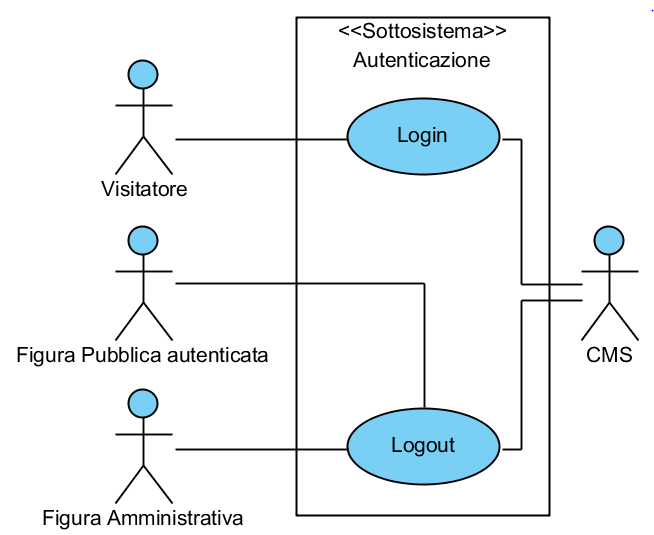
\includegraphics[width=\textwidth]{assets/visualParadigm/Autenticazione}
\end{center}
%*************** LOGIN *****************
\cuTab{cu:login}%
{\getTitletodesc{att:visitatore}}%
{La persona connessa al sito è inizialmente riconosciuta come Visitatore}%
{La persona connessa al sito è ora autenticata, come Utente o Produttore}%
{\begin{enumCU}
	\item Il caso d'uso ha inizio quando un visitatore richiede di effettuare il login 
	\item Il sistema richiede le credenziali di autenticazione 
	\item Il visitatore inserisce le credenziali di accesso negli appositi campi \label{culogin:3}
	\item Il visitatore conferma i dati inseriti
	\item Il sistema verifica che i dati inseriti corrispondano ad un account esistente \label{culogin:5}
	\item Il sistema accetta le credenziali ricevute
\end{enumCU}}%
%
\cuAlternativo{cu:login}
{Flusso alternativo 1}%
{Errore Login}%
{La persona connessa al sito è inizialmente riconosciuta come Visitatore}%
{\postNulle}%
{\begin{enumCU}
	\item Dopo il punto \ref{culogin:5} il sistema rifiuta le credenziali
\end{enumCU}}%
%
\cuAlternativo{cu:login}
{Flusso alternativo 2}%
{Annulla Login}%
{La persona connessa al sito è inizialmente riconosciuta come Visitatore}%
{\postNulle}%
{\begin{enumCU}
		\item Dopo il punto \ref{culogin:3} l'utente annulla l'operazione di login
	\end{enumCU}}%

\tabcuvspace

%*************** LOGOUT *****************
\cuTab{cu:logout}
{\getTitletodesc{att:utente}, \getTitletodesc{att:produttore}}
{La persona connessa al sito è autenticata}
{La persona connessa al sito non è più autenticata, ed è ora un Visitatore}
{\begin{enumCU}
	\item Il caso d'uso ha inizio quando una persona autenticata richiede di effettuare il logout
	\item Il sistema effettua il logout richiesto
\end{enumCU}}

\subsection{Gestione iscrizioni}
\begin{center}
   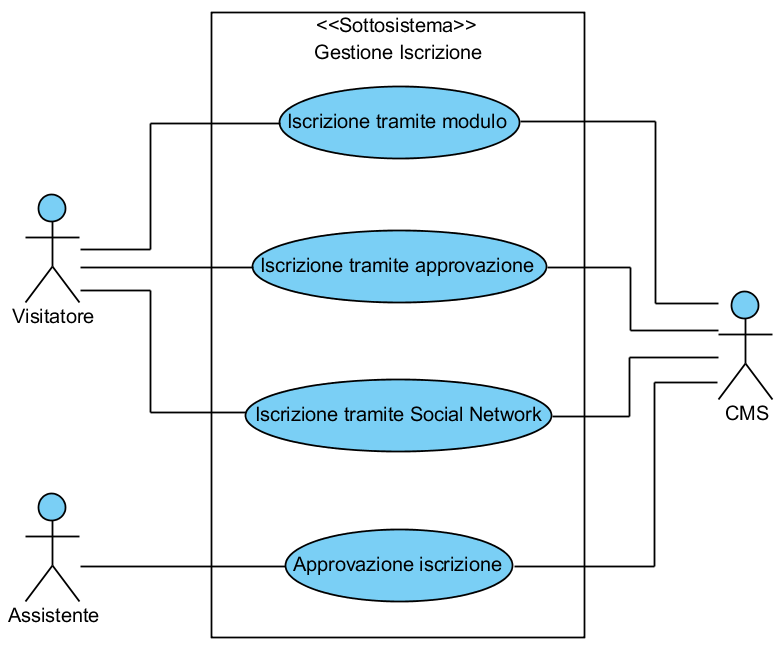
\includegraphics[width=\textwidth]{assets/visualParadigm/GestioneIscrizione}
\end{center}
%*************** ISCRIZIONE PORTALE *****************
\cuTab{cu:iscrizionePortale}
{\getTitletodesc{att:visitatore}}
{La persona connessa al sito è inizialmente riconosciuta come Visitatore}
{La persona ha ora un account proprio, creato con i dati da essa inseriti}
{\begin{enumCU}
	\item Il caso d'uso ha inizio quando un visitatore richiede di effettuare l'iscrizione
	\item Il sistema richiede i dati richiesti per effettuare l'iscrizione
	\item Il visitatore inserisce i dati richiesti negli appositi campi \label{cuiscr:3}
	\item Il visitatore conferma i dati inseriti
	\item Il sistema verifica che i dati inseriti siano corretti e che l'identificatore dell'account che si sta creando non sia già presente \label{cuiscr:5}
	\item Il sistema accetta le credenziali ricevute
\end{enumCU}}
%
\cuAlternativo{cu:iscrizionePortale}
{Flusso alternativo 1}%
{Annulla iscrizione}%
{La persona connessa al sito è inizialmente riconosciuta come Visitatore}%
{\postNulle}%
{\begin{enumCU}
		\item Dopo il punto \ref{cuiscr:3} l'utente annulla l'operazione di iscrizione
	\end{enumCU}}%
%
\cuAlternativo{cu:iscrizionePortale}
{Flusso alternativo 2}%
{Errore iscrizione}%
{La persona connessa al sito è inizialmente riconosciuta come Visitatore}%
{\postNulle}%
{\begin{enumCU}
		\item Dopo il punto \ref{cuiscr:5} il sistema rileva un errore nei dati inseriti
	\end{enumCU}}%


\tabcuvspace

%%%FORSE DA TOGLIERE -------------------------------------------------------------------------
%Accorpa verificati e non verificati
\cuTab{cu:iscrizioneSocial}{\getTitletodesc{att:visitatore}}{La persona è connessa al sito come Visitatore}{La persona ha ora un account proprio, creato tramite le API messe a disposizione dal Social Network utilizzato durante l'iscrizione}{}

\tabcuvspace

%*************** ISCRIZIONE CON APPROVAZIONE *****************
\cuTab{cu:iscrizioneApprovazione}
{\getTitletodesc{att:visitatore}}
{La persona connessa al sito è inizialmente riconosciuta come Visitatore}
{Viene inserita nel sistema una richiesta di creazione di un account di tipo produttore}
{\begin{enumCU}
	\item Il caso d'uso ha inizio quando un visitatore richiede di effettuare l'iscrizione tramite approvazione
	\item Il sistema richiede i dati richiesti per effettuare l'iscrizione
	\item Il visitatore inserisce i dati richiesti negli appositi campi \label{cuiscrapp:3}
	\item Il visitatore conferma i dati inseriti
	\item Il sistema verifica che i dati inseriti siano corretti e che l'identificatore dell'account che si sta creando non sia già presente \label{cuiscrapp:5}
	\item Il sistema accetta le credenziali ricevute 
\end{enumCU}}
%
\cuAlternativo{cu:iscrizioneApprovazione}
{Flusso alternativo 1}%
{Annulla iscrizione}%
{La persona connessa al sito è inizialmente riconosciuta come Visitatore}%
{\postNulle}%
{\begin{enumCU}
		\item Dopo il punto \ref{cuiscrapp:3} l'utente annulla l'operazione di iscrizione
	\end{enumCU}}%
%
\cuAlternativo{cu:iscrizioneApprovazione}
{Flusso alternativo 2}%
{Errore iscrizione}%
{La persona connessa al sito è inizialmente riconosciuta come Visitatore}%
{\postNulle}%
{\begin{enumCU}
		\item Dopo il punto \ref{cuiscrapp:5} il sistema rileva un errore nei dati inseriti
	\end{enumCU}}%

\tabcuvspace

%***************  APPROVAZIONE DI UNA RICHIESTA DI ISCRIZIONE *****************
\cuTab{cu:approvazioneIscrizione}
{\getTitletodesc{att:assistente}}
{La persona connessa al sito è autenticata e ha i privilegi di  Assistente. Nel sistema è presente una richiesta di creazione di un account}
{Il Visitatore che ha effettuato la richiesta ha ora un account di tipo produttore. Nel sistema non è più presente la richesta}
{\begin{enumCU}
	\item Il caso d'uso ha inizio quando una persona con privilegi di assistente controlla una richiesta di creazione di account di tipo produttore \label{cuappriscr:1}
	\item L'assistente approva la richiesta di creazione dell'account
\end{enumCU}}
%
\cuAlternativo{cu:approvazioneIscrizione}
{Flusso alternativo 1}%
{Richiesta rifiutata}%
{La persona connessa al sito è autenticata e ha i privilegi di Assistente}%
{Nel sistema non è più presente la richesta}%
{\begin{enumCU}
		\item Dopo il punto \ref{cuappriscr:1} l'assistente rifiuta la richiesta di creazione dell'account
	\end{enumCU}}%

\subsection{Gestione vetrina}
\begin{center}
   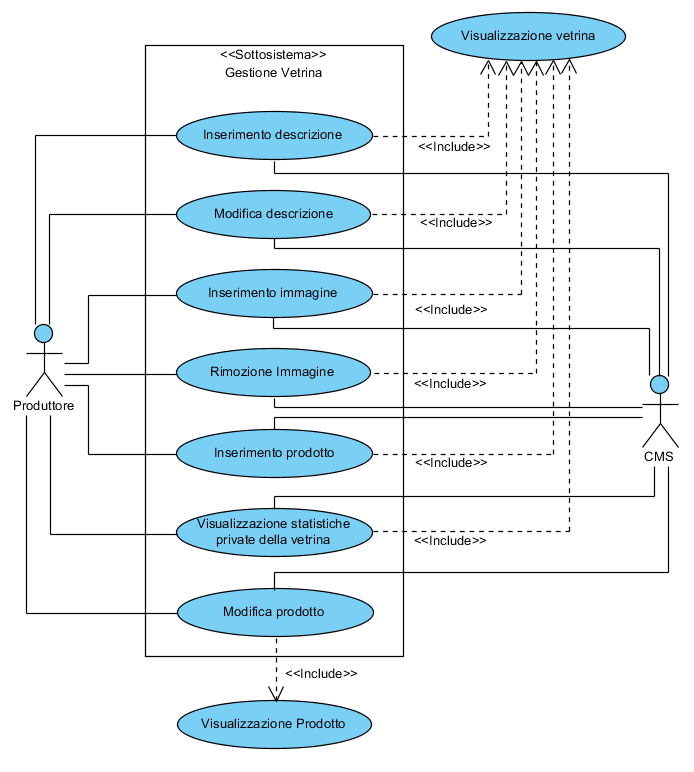
\includegraphics[width=\textwidth]{assets/visualParadigm/GestioneVentrina}
\end{center}
%
%***************  INSERISCI DESCRIZIONE IN VETRINA *****************
\cuTab{cu:personalizzaVetrinaInsDesc}
{\getTitletodesc{att:produttore}}
{La persona connessa al sito è autenticata e ha i privilegi di Produttore}
{Nel sistema è presente la descrizione della vetrina inserita dal Produttore}
{\begin{enumCU}
		\item Il caso d'uso ha inizio quando un produttore richiedere di inserire una descrizione nella vetrina
		\item Il sistema richiede il testo da inserire come descrizione \label{cuinsdescr:2}
		\item Il produttore inserisce la decrizione nell'apposito campo \label{cuinsdescr:3}
		\item Il produttore conferma il testo inserito
		\item Il sistema accetta il testo inserito
	\end{enumCU}}
%
\cuAlternativo{cu:personalizzaVetrinaInsDesc}
{Flusso alternativo 1}%
{Annulla inserimento}%
{La persona connessa al sito è autenticata e ha i privilegi di Produttore}%
{\postNulle}%
{\begin{enumCU}
		\item Dopo il punto \ref{cuinsdescr:2} il produttore annulla l'inserimento della descrizione
	\end{enumCU}}%
%
\cuAlternativo{cu:personalizzaVetrinaInsDesc}
{Flusso alternativo 2}%
{Modifica descrizione}%
{La persona connessa al sito è autenticata e ha i privilegi di Produttore. Nel sistema è già presente una descrizione della vetrina}%
{Nel sistema è la descrizione della vetrina è stata correttamente modificata}%
{\begin{enumCU}
		\item Nel punto \ref{cuinsdescr:3} il sistema chiede di inserire la descrizione, il campo è precompilato con la descrizione attuale
	\end{enumCU}}%

\tabcuvspace

%***************  INSERISCI IMMAGINE IN VETRINA *****************
\cuTab{cu:personalizzaVetrinaInsImg}
{\getTitletodesc{att:produttore}}
{La persona connessa al sito è autenticata e ha i privilegi di Produttore}
{Nel sistema è presente l'immagine della vetrina inserita dal Produttore}
{\begin{enumCU}
		\item Il caso d'uso ha inizio quando un produttore richiedere di inserire un immagine nella vetrina
		\item Il sistema richiede il percorso nel file system dell'immagine da inserire 
		\item Il produttore inserisce il percorso dell'immagine nell'apposito campo \label{cuinsimm:2}
		\item Il produttore conferma il percorso dell'immagine inserito \label{cuinsimm:3}
		\item Il sistema accetta il percorso dell'immagine inserito e salva l'immagine nel sistema
	\end{enumCU}}
%
\cuAlternativo{cu:personalizzaVetrinaInsImg}
{Flusso alternativo 1}%
{Errore inserimento}%
{La persona connessa al sito è autenticata e ha i privilegi di Produttore}%
{\postNulle}%
{\begin{enumCU}
		\item Dopo il punto \ref{cuinsimm:3} il sistema non riesce a trovare, caricare o inserire correttamente l'immagine
	\end{enumCU}}%
%
\cuAlternativo{cu:personalizzaVetrinaInsImg}
{Flusso alternativo 2}%
{Anulla inserimento}%
{La persona connessa al sito è autenticata e ha i privilegi di Produttore}%
{\postNulle}%
{\begin{enumCU}
		\item Dopo il punto \ref{cuinsimm:2} il produttore annulla l'inserimento dell'immagine
	\end{enumCU}}%

\tabcuvspace

%***************  INSERISCI PRODOTTO IN VETRINA *****************
\cuTab{cu:personalizzaVetrinaInsProd}
{\getTitletodesc{att:produttore}}
{La persona connessa al sito è autenticata e ha i privilegi di Produttore}
{Nel sistema è presente il prodotto che Produttore ha inserito in vetrina}
{\begin{enumCU}
		\item Il caso d'uso ha inizio quando un produttore richiedere di inserire un prodotto nella vetrina
		\item Il sistema richiede di compilare la scheda del prodotto da inserire
		\item Il produttore inserisce i dati richiesti \label{cuinsimmpro:1}
		\item Il produttore conferma i dati inseriti 
		\item Il sistema richiede uno o più percorsi nel file system delle immagini del prodotto da inserire
		\item Il produttore inserisce nell'apposito campo uno o più percorsi nel file system delle immagini che vuole inserire \label{cuinsimmpro:2}
		\item Il produttore conferma i percorsi inseriti \label{cuinsimmpro:3}
		\item Il sistema accetta i dati inseriti e i percorsi inseriti e salva le immagini nel sistema
	\end{enumCU}}
%
\cuAlternativo{cu:personalizzaVetrinaInsProd}
{Flusso alternativo 1}%
{Errore inserimento}%
{La persona connessa al sito è autenticata e ha i privilegi di Produttore}%
{\postNulle}%
{\begin{enumCU}
		\item Dopo il punto \ref{cuinsimmpro:3} il sistema non riesce a trovare, caricare o inserire correttamente una o più immagini
	\end{enumCU}}%
%
\cuAlternativo{cu:personalizzaVetrinaInsProd}
{Flusso alternativo 2}%
{Anulla inserimento}%
{La persona connessa al sito è autenticata e ha i privilegi di Produttore}%
{\postNulle}%
{\begin{enumCU}
		\item Dopo il punto \ref{cuinsimmpro:2} o dopo il punto \ref{cuinsimmpro:1} il produttore annulla l'inserimento del prodotto
	\end{enumCU}}%

\tabcuvspace

%***************  MODIFICA PRODOTTO IN VETRINA *****************
\cuTab{cu:personalizzaVetrinaModProd}
{\getTitletodesc{att:produttore}}
{La persona connessa al sito è autenticata e ha i privilegi di Produttore. Il prodotto è presente nella sua vetrina}%
{Nel sistema il prodotto è stato correttamente modificato}
{\begin{enumCU}
		\item Il caso d'uso ha inizio quando un produttore richiede di modificare un prodotto presente nella sua vetrina
		\item Il sistema richiede di compilare la scheda prodotto, percompilata con i dati già presenti nel sistema
		\item Il produttore inserisce i dati richiesti \label{cumodprodelim:1}
		\item Il produttore conferma i dati inseriti
		\item Il sistema mostra le immagini del prodotto presenti, con la possibilità di eliminarle, e mostra i campi per aggiungere i percorsi nel file system di altre immagini da aggiungere \label{cumodprodelim:3}
		\item Il produttore inserisce i percorsi nel file system delle immagini che intende aggiungere
		\item Il produttore conferma i percorsi inseriti \label{cumodprodelim:2}
		\item Il sistema accetta i dati inseriti e i percorsi inseriti e salva le immagini nel sistema
	\end{enumCU}} %%SETTARE UN PRODOTTO COME FUORI PRODUZIONE&&
%
\cuAlternativo{cu:personalizzaVetrinaModProd}
{Flusso alternativo 1}%
{Elimina immagine}%
{La persona connessa al sito è autenticata e ha i privilegi di Produttore. Il prodotto è presente nella sua vetrina}
{L'immagine selezionata non è più presente nel sistema}%
{\begin{enumCU}
		\item Dopo il punto \ref{cumodprodelim:3} il produttore decide di eliminare un immagine
		\item Il sistema elimina l'immagine dal sistema
	\end{enumCU}}%
%
\cuAlternativo{cu:personalizzaVetrinaModProd}
{Flusso alternativo 2}%
{Anulla Modifica}%
{La persona connessa al sito è autenticata e ha i privilegi di Produttore. Il prodotto è presente nella sua vetrina}%
{\postNulle}%
{\begin{enumCU}
		\item Dopo il punto \ref{cumodprodelim:2} o dopo il punto \ref{cumodprodelim:1} il produttore annulla l'inserimento del prodotto
	\end{enumCU}}%

\tabcuvspace

%***************  STATISTICHE PRIVATE VETRINA *****************
\cuTab{cu:statistichePrivateVetrina}
{\getTitletodesc{att:produttore}}
{La persona connessa al sito è autenticata e ha i privilegi di Produttore}
{Il Produttore accede alle statistiche private della propria vetrina}
{\begin{enumCU}
		\item Il caso d'uso ha inizio quando un produttore richiede di accedere alle statistiche private della sua vetrina
		\item Il sistema mostra al produttore le statistiche della sua vetrina
	\end{enumCU}}


\subsection{Gestione notizie}
\begin{center}
   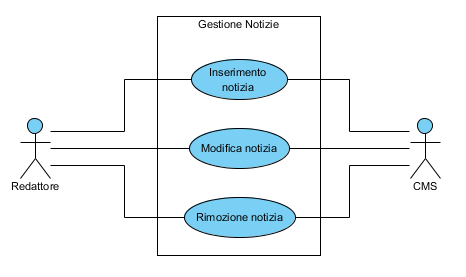
\includegraphics[width=\textwidth]{assets/visualParadigm/GestioneNotizie}
\end{center}
%
%***************  INSERIMENTO NOTIZIA *****************
\cuTab{cu:inserimentoNotizia}
{\getTitletodesc{att:redattore}}
{La persona connessa al sito è autenticata e ha i privilegi di Redattore}
{Nel  sistema è presente la notizia inserita dal Redattore}
{\begin{enumCU}
	\item Il caso d'uso ha inizio quando un redattore richiede di inserire una notizia  
	\item Il sistema richiede di compilare i campi necessari all'inserimento della notizia
	\item Il redattore inserisce i dati richiesti \label{cuinsnot:2}
	\item Il redattore conferma i dati richiesti
	\item Il sistema accetta i dati inseriti e crea una nuova notizia nel sistema
\end{enumCU}}
%
\cuAlternativo{cu:inserimentoNotizia}
{Flusso alternativo 1}%
{Anulla inserimento}%
{La persona connessa al sito è autenticata e ha i privilegi di Redattore}%
{\postNulle}%
{\begin{enumCU}
		\item Dopo il punto \ref{cuinsnot:2} il redattore annulla l'inserimento della notizia
	\end{enumCU}}%

\tabcuvspace

%***************  MODIFICA NOTIZIA *****************
\cuTab{cu:modificaNotizia}
{\getTitletodesc{att:redattore}}
{La persona è autenticata e ha i privilegi di Redattore. La notizia è presente nel sistema}
{La notizia è stata correttamente modificata}
{\begin{enumCU}
	\item Il caso d'uso ha inizio quando un redattore richiede di modificare una notizia presente nel sistema 
	\item Il sistema mostra i campi necessari all'inserimento della notizia precompilati con i dati già presenti nel sistema
	\item Il redattore inserisce, modifica o lascia inalterati i dati richiesti \label{cumodnot:2}
	\item Il redattore conferma i dati richiesti
	\item Il sistema accetta i dati inseriti e modifica la notizia nel sistema
\end{enumCU}}
%
\cuAlternativo{cu:modificaNotizia}
{Flusso alternativo 1}%
{Anulla modifica}%
{La persona connessa al sito è autenticata e ha i privilegi di Redattore}%
{\postNulle}%
{\begin{enumCU}
		\item Dopo il punto \ref{cumodnot:2} il redattore annulla la modifica della notizia
	\end{enumCU}}%

\tabcuvspace

%***************  RIMOZIONE NOTIZIA *****************
\cuTab{cu:rimozioneNotizia}
{\getTitletodesc{att:redattore}}
{La persona è autenticata e ha i privilegi di Redattore. La notizia è presente nel sistema}
{Nel sistema non è più presente la notizia eliminata}
{\begin{enumCU}
	\item Il caso d'uso ha inizio quando un redattore richiede di eliminare una notizia presente nel sistema
	\item Il sistema chiede conferma dell'eliminazione \label{curemnot:2}
	\item Il redattore conferma l'eliminazione
\end{enumCU}}
%
\cuAlternativo{cu:rimozioneNotizia}
{Flusso alternativo 1}%
{Anulla rimozione}%
{La persona connessa al sito è autenticata e ha i privilegi di Redattore}%
{\postNulle}%
{\begin{enumCU}
		\item Dopo il punto \ref{curemnot:2} il redattore annulla la rimozione della notizia
	\end{enumCU}}%


\subsection{Gestione suggerimenti}
\begin{center}
   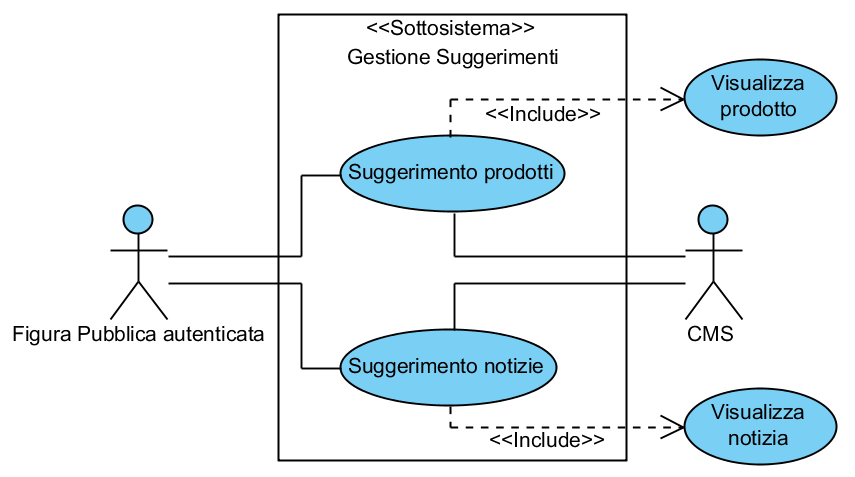
\includegraphics[width=\textwidth]{assets/visualParadigm/GestioneSuggerimenti}
\end{center}
%***************  SUGGERIMENTO PRODOTTI *****************
%Accorpa suggerimento intelligente e simili
\cuTab{cu:suggerimentoProdotti}{\getTitletodesc{att:utente}, \getTitletodesc{att:produttore}}{La persona è autenticata nel sistema e sta visualizzando un prodotto}{Viene suggerito un prodotto presente nel sistema}{}

\tabcuvspace

\cuTab{cu:notizieSimili}{\getTitletodesc{att:utente}, \getTitletodesc{att:produttore}}{La persona è autenticata nel sistema e sta visualizzando una notizia}{Viene suggerita una notizia presente nel sistema}{}

\subsection{Gestione account}
\begin{center}
   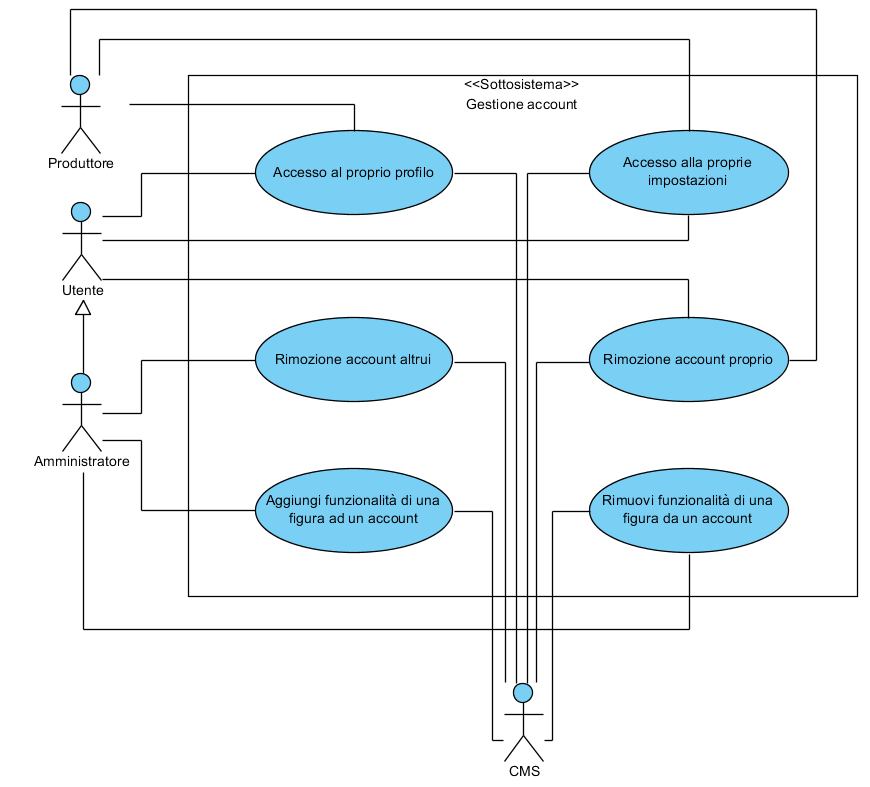
\includegraphics[width=\textwidth]{assets/visualParadigm/GestioneAccount}
\end{center}
\cuTab{cu:accessoProfilo}{\getTitletodesc{att:utente}, \getTitletodesc{att:produttore}}{La persona è autenticata nel sistema}{La persona visualizza il suo profilo}{}

\tabcuvspace

\cuTab{cu:accessoImpostazioni}{\getTitletodesc{att:utente}, \getTitletodesc{att:produttore}}{La persona è autenticata nel sistema}{La persona visualizza la pagina delle proprie impostazioni}{}

\tabcuvspace

\cuTab{cu:rimozioneAccountProprio}{\getTitletodesc{att:utente}, \getTitletodesc{att:produttore}}{La persona è autenticata nel sistema}{L'account della persona non è più presente nel sistema}{}

\tabcuvspace

\cuTab{cu:rimozioneAccountAltrui}{\getTitletodesc{att:amministratore}}{La persona è autenticata e ha i privilegi di Amministratore. L'account da rimuovere è presente nel sistema}{L'account da rimuovere non è più presente nel sistema}{}

\tabcuvspace

\cuTab{cu:aggiungiAccountAFigura}{\getTitletodesc{att:amministratore}}{La persona è autenticata e ha i privilegi di Amministratore. L'account da modificare è presente nel sistema e non ha già i privilegi della figura scelta}{L'account da modificare ha i privilegi della figura scelta, oltre a quelli già posseduti}{}

\tabcuvspace

\cuTab{cu:rimuoviAccountDaFigura}{\getTitletodesc{att:amministratore}}{La persona è autenticata e ha i privilegi di Amministratore. L'account da modificare è presente nel sistema e ha già i privilegi della figura scelta}{L'account da modificare non ha più i privilegi della figura scelta, ma mantiene gli altri}{}


\subsection{Gestione valutazioni}
\begin{center}
   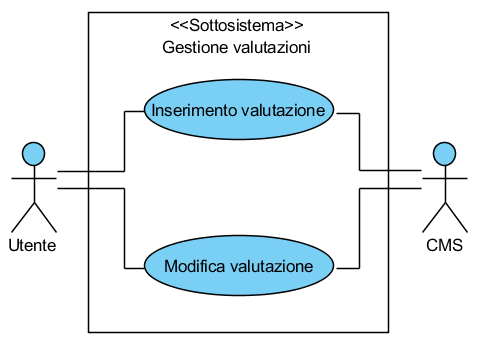
\includegraphics[width=\textwidth]{assets/visualParadigm/GestioneValutazioni}
\end{center}
\cuTab{cu:inserisciValutazioneProdotto}{\getTitletodesc{att:utente}}{La persona è autenticata come Utente. Il prodotto è presente nel sistema}{La valutazione dell'Utente per quel prodotto è aggiunta nel sistema}{}

\tabcuvspace

\cuTab{cu:modificaValutazioneProdotto}{\getTitletodesc{att:utente}}{La persona è autenticata come Utente e ha effettuato una valutazione di un prodotto presente nel sistema}{La valutazione viene modificata correttamente}{}


\subsection{Gestione recensioni}
\begin{center}
   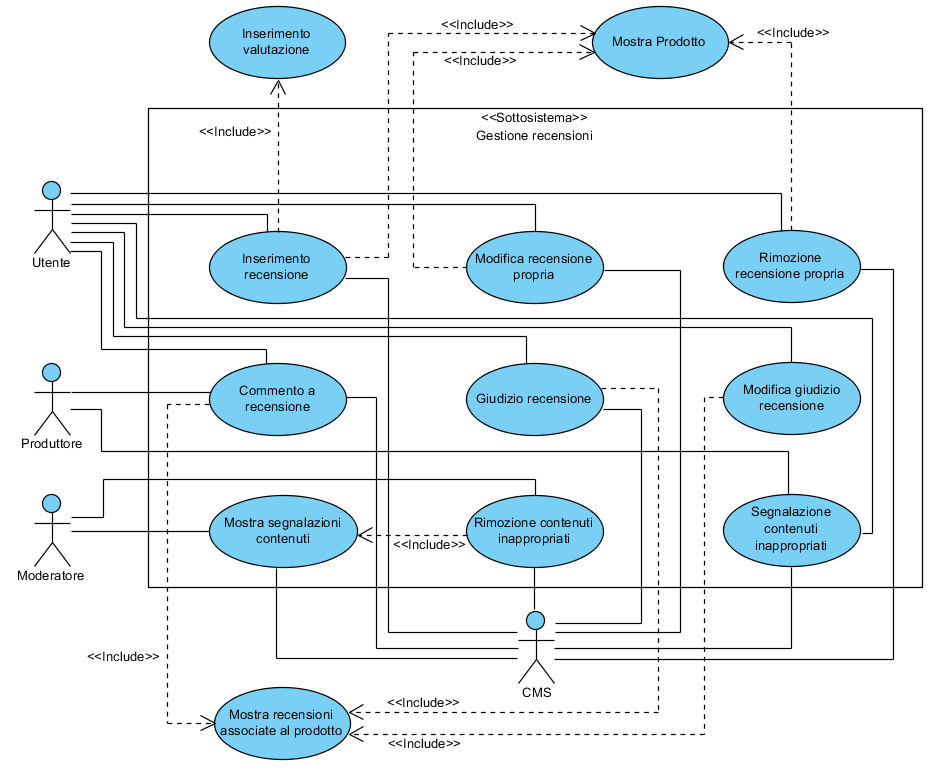
\includegraphics[width=\textwidth]{assets/visualParadigm/GestioneRecensioni}
\end{center}
\cuTab{cu:inserisciRecensioneProdotto}{\getTitletodesc{att:utente}}{La persona è autenticata come Utente. Il prodotto è presente nel sistema e non è già stato recensito dall'Utente}{La recensione dell'Utente per quel prodotto è aggiunta nel sistema}{}

\tabcuvspace

\cuTab{cu:modificaRecensioneProdotto}{\getTitletodesc{att:utente}}{La persona è autenticata come Utente e ha effettuato una recensione di un prodotto presente nel sistema}{La recensione viene modificata correttamente}{}

\tabcuvspace

\cuTab{cu:eliminaRecensioneProdotto}{\getTitletodesc{att:utente}}{La persona è autenticata come Utente e ha effettuato una recensione di un prodotto presente nel sistema}{La recensione viene eliminata correttamente}{}

\tabcuvspace

\cuTab{cu:commentoRecensione}{\getTitletodesc{att:utente}, \getTitletodesc{att:produttore}}{La persona è autenticata come Utente o come Produttore. La recensione di un prodotto è presente nel sistema}{Il commento viene aggiunto ai commenti di quella recensione}{}

\tabcuvspace

\cuTab{cu:giudizioRecensione}{\getTitletodesc{att:utente}}{La persona è autenticata come Utente. La recensione di un prodotto è presente nel sistema}{Il giudizio (positivo o negativo) per quella recensione viene aggiunto nel sistema}{}

\tabcuvspace

\cuTab{cu:segnalazioneContenutiInap}{\getTitletodesc{att:utente}, \getTitletodesc{att:produttore}}{La persona è autenticata come Utente o come Produttore. Il contenuto è presente nel sistema}{La segnalazione viene inviata correttamente al Moderatore}{}

\tabcuvspace

\cuTab{cu:visualizzazioneSegnContenutiInap}{\getTitletodesc{att:moderatore}}{La persona è autenticata ed ha i privilegi Moderatore. La segnalazione è presente nel sistema}{La segnalazione è stata gestita dal Moderatore}{}
%marcare segfnalazione come risolta/eliminarla dalla lista

\tabcuvspace

\cuTab{cu:rimozioneContenutiInap}{\getTitletodesc{att:moderatore}}{La persona è autenticata ed ha i privilegi Moderatore. Il contenuto da rimuovere è presente nel sistema}{Il contenuto da rimuovere non è più presente nel sistema}{}


\subsection{Interazione tra figure}
\begin{center}
   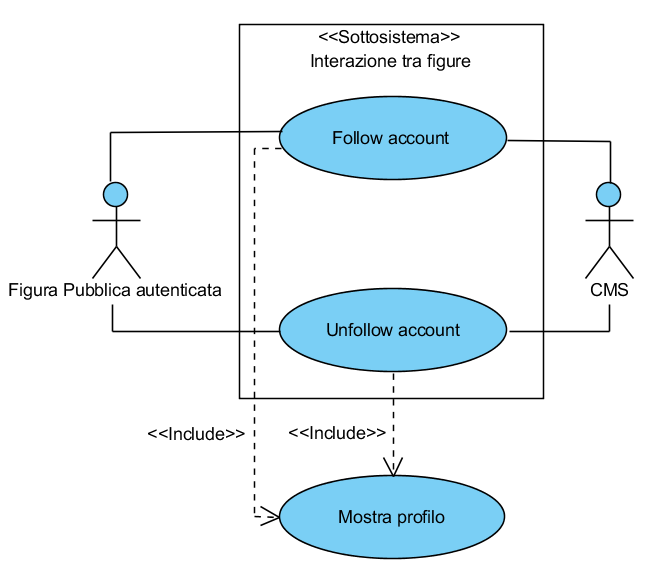
\includegraphics[width=\textwidth]{assets/visualParadigm/InterazioneTraFigure}
\end{center}
\cuTab{cu:followAccount}{\getTitletodesc{att:utente}, \getTitletodesc{att:produttore}}{La persona è autenticata come Utente o come Produttore. L'account da seguire è presente nel sistema}{L'account da seguire viene aggiunto alla lista degli account che si seguono}{}

\tabcuvspace

\cuTab{cu:unFollowAccount}{\getTitletodesc{att:utente}, \getTitletodesc{att:produttore}}{La persona è autenticata come Utente o come Produttore. L'account seguito è presente nel sistema}{L'account seguito viene rimosso dalla lista degli account che si seguono}{}


\subsection{Gestione ticket}
\begin{center}
   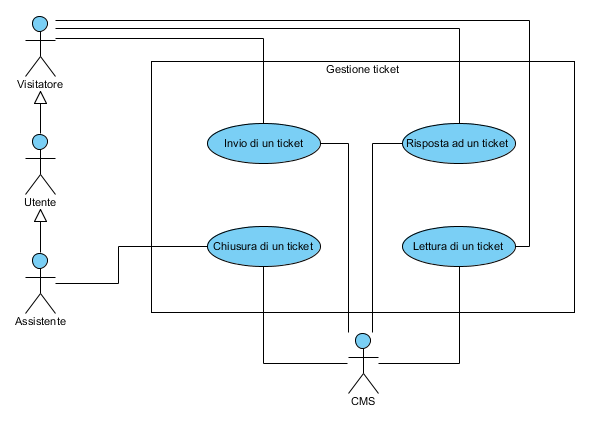
\includegraphics[width=\textwidth]{assets/visualParadigm/GestioneTicket}
\end{center}
\cuTab{cu:ticketInvio}{\getTitletodesc{att:utente}, \getTitletodesc{att:produttore}}{La persona è autenticata come Utente o come Produttore}{Viene creato un nuovo ticket}{}

\tabcuvspace

\cuTab{cu:ticketRisposta}{\getTitletodesc{att:utente}, \getTitletodesc{att:produttore}, \getTitletodesc{att:assistente}}{La persona è autenticata come Utente o come Produttore o ha i privilegi di Assistente. Il ticket è stato creato da quella persona}{La risposta al ticket è aggiunta nel sistema}{}

\tabcuvspace

\cuTab{cu:ticketChiudi}{\getTitletodesc{att:assistente}}{La persona è autenticata e ha i privilegi di Assistente. Il ticket è presente nel sistema}{Il ticket viene etichettato come chiuso}{}

\tabcuvspace

\cuTab{cu:ticketLettura}{\getTitletodesc{att:utente}, \getTitletodesc{att:produttore}, \getTitletodesc{att:assistente}}{La persona è autenticata come Utente o come Produttore o ha i privilegi di Assistente. Il ticket è stato creato da quella persona}{Il ticket viene visualizzato}{}


\subsection{Ricerca contenuti}
\begin{center}
   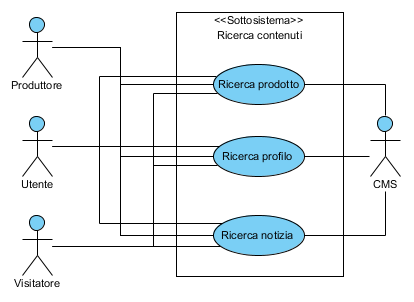
\includegraphics[width=\textwidth]{assets/visualParadigm/RicercaContenuti}
\end{center}
\cuTab{cu:ricercaProdotto}{\getTitletodesc{att:visitatore}, \getTitletodesc{att:utente}, \getTitletodesc{att:produttore}}{-}{I risultati della ricerca sono visualizzati}{}

\tabcuvspace

\cuTab{cu:ricercaProfilo}{\getTitletodesc{att:visitatore}, \getTitletodesc{att:utente}, \getTitletodesc{att:produttore}}{-}{I risultati della ricerca sono visualizzati}{}

\tabcuvspace

\cuTab{cu:ricercaNotizia}{\getTitletodesc{att:visitatore}, \getTitletodesc{att:utente}, \getTitletodesc{att:produttore}}{-}{I risultati della ricerca sono visualizzati}{}


\subsection{Gestione prodotti mancanti}
\begin{center}
   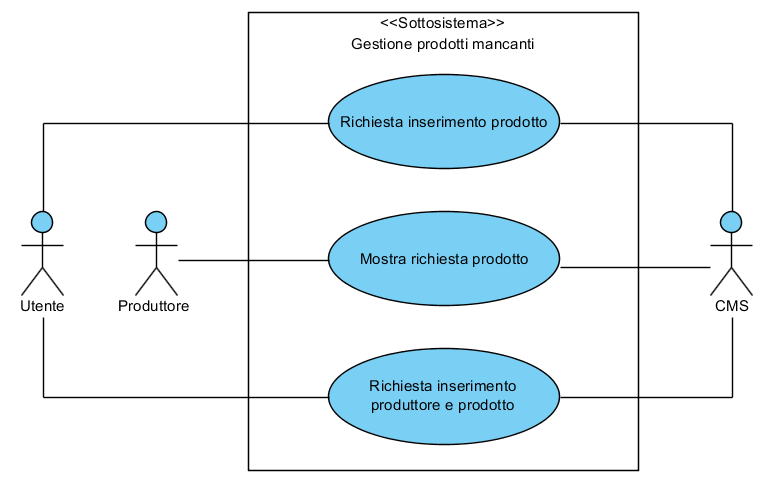
\includegraphics[width=\textwidth]{assets/visualParadigm/GestioneProdottiMancanti}
\end{center}
\cuTab{cu:richiestaInsProdotto}{\getTitletodesc{att:utente}}{La persona è autenticata come Utente. Il Produttore è presente nel sistema. Il prodotto non è presente nel sistema}{La richiesta è inviata al Produttore}{}

\tabcuvspace

\cuTab{cu:visualizzazioneRichiestaInsProdotto}{\getTitletodesc{att:produttore}}{La persona è autenticata come Produttore. La richiesta è presente nel sistema}{La richiesta è stata gestita dal Produttore}{}

\tabcuvspace

\cuTab{cu:richiestaInsProduttore}{\getTitletodesc{att:utente}}{La persona è autenticata come Utente. Il Produttore non è presente nel sistema}{La richiesta è inviata all'assistente tramite ticket}{}


\subsection{Visualizzazione contenuti pubblici}
\begin{center}
   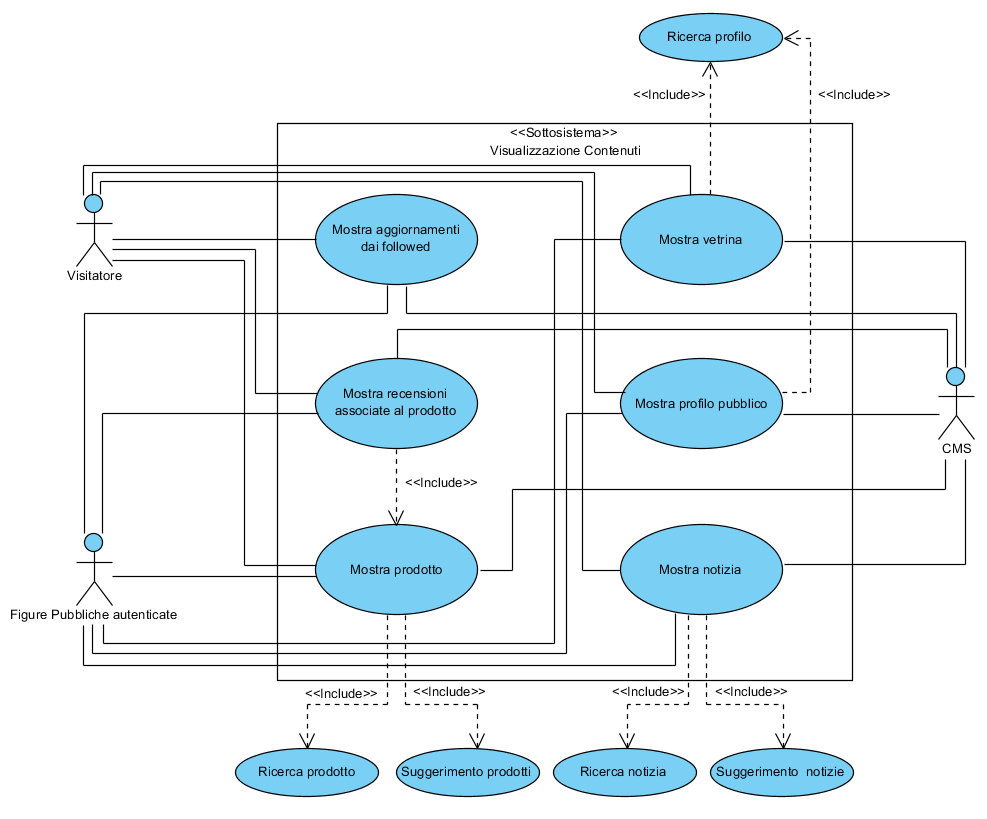
\includegraphics[width=\textwidth]{assets/visualParadigm/Visualizzazione}
\end{center}
%accorpa visalizza prodotti in vetrina e visualizza vetrina
\cuTab{cu:visualizzazioneVetrina}{\getTitletodesc{att:visitatore}, \getTitletodesc{att:utente}, \getTitletodesc{att:produttore}}{La vetrina è presente nel sistema}{La vetrina è mostrata}{}

\tabcuvspace

%Cambiato da: statistiche pubbliche vetrina
\cuTab{cu:visualizzazioneInfoVetrina}{\getTitletodesc{att:visitatore}, \getTitletodesc{att:utente}, \getTitletodesc{att:produttore}}{La vetrina è presente nel sistema}{Le informazioni relative alla vetrina sono mostrate}{}

%\tabcuvspace
%
%\cuTab{cu:visualizzazioneProdottiVetrina}{\getTitletodesc{att:visitatore}, \getTitletodesc{att:utente}, \getTitletodesc{att:produttore}}{}{}{}

\tabcuvspace

\cuTab{cu:visualizzazioneProdotto}{\getTitletodesc{att:visitatore}, \getTitletodesc{att:utente}, \getTitletodesc{att:produttore}}{Il prodotto è presente nel sistema}{Il prodotto è mostrato}{}

\tabcuvspace

%Accorpa statistiche prodotto e informazioni prodotto
\cuTab{cu:visualizzazioneInfoProdotto}{\getTitletodesc{att:visitatore}, \getTitletodesc{att:utente}, \getTitletodesc{att:produttore}}{Il prodotto è presente nel sistema}{Le informazioni e le statistiche relative al prodotto sono mostrate}{}

\tabcuvspace

\cuTab{cu:visualizzazioneRecProdotto}{\getTitletodesc{att:visitatore}, \getTitletodesc{att:utente}, \getTitletodesc{att:produttore}}{Il prodotto è presente nel sistema}{Le recensioni relative al prodotto sono mostrate}{}

\tabcuvspace

%\cuTab{cu:visualizzazioneStatProdotto}{\getTitletodesc{att:visitatore}, \getTitletodesc{att:utente}, \getTitletodesc{att:produttore}}{}{}{}
%
%\tabcuvspace

\cuTab{cu:visualizzazioneProfilo}{\getTitletodesc{att:visitatore}, \getTitletodesc{att:utente}, \getTitletodesc{att:produttore}}{Il profilo è presente nel sistema}{Il profilo è mostrato}{}

\tabcuvspace

%Accorpa informazioni profilo e statistiche profilo
\cuTab{cu:visualizzazioneInfoProfilo}{\getTitletodesc{att:visitatore}, \getTitletodesc{att:utente}, \getTitletodesc{att:produttore}}{Il profilo è presente nel sistema}{Le informazioni e le statistiche relative al profilo sono mostrate}{}

%\tabcuvspace
%
%\cuTab{cu:visualizzazioneStatProfilo}{\getTitletodesc{att:visitatore}, \getTitletodesc{att:utente}, \getTitletodesc{att:produttore}}{}{}{}

\tabcuvspace

\cuTab{cu:visualizzazioneNotizia}{\getTitletodesc{att:visitatore}, \getTitletodesc{att:utente}, \getTitletodesc{att:produttore}}{La notizia è presente nel sistema}{La notizia è mostrata}{}

\tabcuvspace

\cuTab{cu:visualizzazioneAggF}{\getTitletodesc{att:utente}, \getTitletodesc{att:produttore}}{La persona è autenticata come Utente o come Produttore}{Vengono mostrati gli aggiornamenti delle persone che si stanno seguendo}{}




























%Struttura dei casi d'uso (ID) T_T
%Esempi:
%Lumiere -> Ogni caso `e identificato da una stringa del tipo CU.entit`a.sottoentit`a.caso.
%Airbnb.it -> package = PKG_<numero package>_<numero_sottopackage> | caso d'uso = UC_<numero package>_<numero caso d’uso> | attore = ATT_<num. Attore generico>_<num. Attore specifico>

%A me la struttura a package piace, possiamo racchiudere molti casi d'uso in categorie così.

%Scopiazzerei il grafico di Airbnb.it a pagina 9, utilizzando quella figura per descrivere il sistema a grandi linee, con i package. Mostrata questa, procederei con l'analisi
%dei package uno ad uno e quindi dei singoli casi d'uso.
%Per ogni caso d'uso, entrambi gli esempi fanno la descrizione stile Basi 2 con precondizioni e postcondizioni (oltre che attori coinvolti, nome, descrizione e flusso).
%A me piace


